\documentclass{beamer}

%----------------------------------------------------------------------------------------
%	PACKAGES
%----------------------------------------------------------------------------------------
\usepackage{caption}
\usepackage{amsmath}
\usepackage{amssymb}
\usepackage{tikz}
\usetikzlibrary{matrix,backgrounds,arrows,decorations.markings}
\tikzset{
  big arrow/.style={
    decoration={markings,mark=at position 1 with {\arrow[scale=2,#1]{>}}},
    postaction={decorate},
    shorten >=0.4pt,
    dashed=true},
  big arrow/.default=red,
  }
\usepackage{minted}
\usepackage[numbers]{natbib}
\bibliographystyle{IEEEtran}

\usepackage{outlines} % Nested itemize lists
\usepackage{stmaryrd} % For llbracket, rrbracket
\usepackage[super]{nth} % For 0th, 1st, 2nd, 3rd, etc., formatting
%----------------------------------------------------------------------------------------

\mode<presentation> {
\usetheme{Montpellier}

\setbeamertemplate{footline}{
  \leavevmode%
  \hbox{%
  \begin{beamercolorbox}[wd=.4\paperwidth,ht=2.25ex,dp=1ex,center]{mb2244}%
    \usebeamerfont{mb2244}\insertshortauthor
  \end{beamercolorbox}%
  \begin{beamercolorbox}[wd=.8\paperwidth,ht=2.25ex,dp=1ex,center]{title in head/foot}%
    \insertframenumber{} / \inserttotalframenumber\hspace*{1ex}
  \end{beamercolorbox}}%
  \vskip0pt%
}

% Remove the navigation symbols from the bottom slides
\setbeamertemplate{navigation symbols}{}
}

%----------------------------------------------------------------------------------------
%	TITLE PAGE
%----------------------------------------------------------------------------------------

\title{Collapsing Heterogeneous Towers of Interpreters}

\author[mb2244]{Michael Buch -- mb2244}
\institute
{
University of Cambridge\\ % Your institution for the title page
\medskip
}
\date{\today} % Date, can be changed to a custom date

\begin{document}

\begin{frame}
\titlepage % Print the title page as the first slide
\end{frame}

\begin{frame}
\frametitle{Overview} % Table of contents slide, comment this block out to remove it
\tableofcontents % Throughout your presentation, if you choose to use \section{} and \subsection{} commands, these will automatically be printed on this slide as an overview of your presentation
\end{frame}

% Show table of contents on section change
\AtBeginSection[]
{
\begin{frame}{Table of Contents}
\tableofcontents[currentsection]
\end{frame}
}

\newcommand{\mslang}{$\lambda_{\uparrow\downarrow}$}
\newcommand{\mevl}{$M_e$}

%----------------------------------------------------------------------------------------
%	PRESENTATION SLIDES
%----------------------------------------------------------------------------------------
\section{Towers}
\begin{frame}{What are they?}
  \begin{columns}
    \begin{column}{0.5\textwidth}
      \begin{itemize}
        \item Reflective Towers
        \item Model for reflection
        \item Used for reflective languages, e.g., 3-LISP \cite{smith1984reflection}, Brown \cite{wand1988mystery}, Blond \cite{danvy1988intensions}
        \item \textbf{n-fold interpretative overhead}
      \end{itemize}
    \end{column}
    \begin{column}{0.5\textwidth}
      \begin{figure}
        \centering
        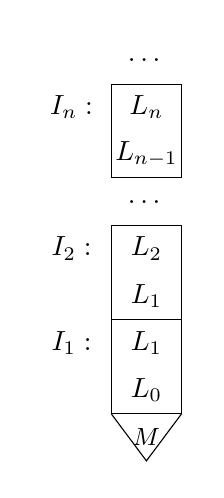
\begin{tikzpicture}
          \matrix (m) [matrix of nodes,nodes={minimum width=2.5em,minimum  height=1.7em},ampersand replacement=\&]
            {
                        \& \dots                   \\
                $I_n:$  \& $L_n$                   \\
                        \& $L_{n-1}$               \\
                        \& \dots                   \\
                $I_2:$  \& $L_2$                   \\
                        \& $L_1$                   \\
                $I_1:$  \& $L_1$                   \\
                        \& $L_0$                   \\
                        \& |[font=\small]|$M$      \\
              };
              \draw (m-1-2.south west) |- (m-4-2.north east) |- (m-1-2.south west);
              \draw (m-4-2.south west) |- (m-6-2.south east) |- (m-4-2.south west);
              \draw (m-4-2.south west) |- (m-8-2.south east) |- (m-6-2.north east);
              \draw (m-8-2.south west) -- (m-9-2.south) -- (m-8-2.south east);
        \end{tikzpicture}
      \end{figure}
    \end{column}
  \end{columns}
\end{frame}

\begin{frame}{Removing Interpretative Overhead}
    \begin{columns}
    \begin{column}{0.5\textwidth}
        \begin{figure}
        \centering
        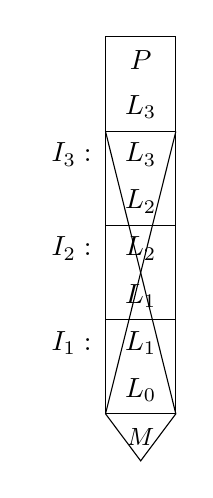
\begin{tikzpicture}
          \matrix (m) [matrix of nodes,nodes={minimum width=2.5em,minimum  height=1.7em},ampersand replacement=\&]
            {
                        \& $P$                      \\
                        \& $L_3$                    \\
                $I_3:$  \& $L_3$                    \\
                        \& $L_2$                    \\
                $I_2:$  \& $L_2$                    \\
                        \& $L_1$                    \\
                $I_1:$  \& $L_1$                    \\
                        \& $L_0$                    \\
                        \& |[font=\small]|$M$       \\
              };
              \draw (m-1-2.north west) |- (m-8-2.south east) |- (m-1-2.north west);
              \draw (m-2-2.south west) -- (m-2-2.south east);
              \draw (m-4-2.south west) -- (m-4-2.south east);
              \draw (m-6-2.south west) -- (m-6-2.south east);
              \draw (m-8-2.south west) -- (m-9-2.south) -- (m-8-2.south east);

              \onslide<2->{
                  \draw (m-2-2.south west) -- (m-8-2.south east);
                  \draw (m-2-2.south east) -- (m-8-2.south west);
                }
        \end{tikzpicture}
        \end{figure}
    \end{column}
    \begin{column}{0.5\textwidth}
        \begin{outline}
            \1 Which combination of $I_1$, $I_2$, $I_3$ to remove?
                \2 Best case: simply run $P$ on $M$
            \onslide<2->{
                \1 Idea: generate new tower without $I_1$ to $I_3$
                    \onslide<3->{
                        \2 Possible solution: turn interpretation into compilation
                    }
            }
            \end{outline}
    \end{column}
  \end{columns}
\end{frame}

\begin{frame}{Motivating Example}
  \begin{columns}
    \begin{column}{0.7\textwidth}
      \begin{outline}
        \1 Python on x86 JavaScript emulator
        \1 Compared to reflective towers:
            \2 \textit{Different internal structure}, e.g., translation to bytecode
            \2 \textit{Different language} at each level
            \onslide<2->{
                \3 Need some way of expressing this \textbf{generalization}
            }
      \end{outline}
    \end{column}
    \begin{column}{0.3\textwidth}
      \begin{figure}
        \centering
        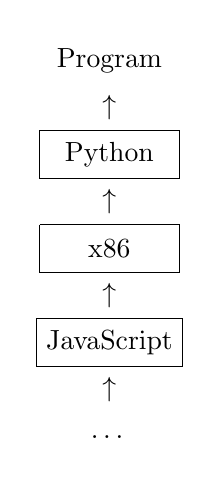
\begin{tikzpicture}
          \matrix (m) [matrix of nodes,nodes={minimum width=5em,minimum  height=1.7em},ampersand replacement=\&]
            {
              Program                   \\
              $\uparrow$                \\
              Python                    \\
              $\uparrow$                \\
              x86                       \\
              $\uparrow$                \\
              JavaScript                \\
              $\uparrow$                \\
              \dots                     \\
              };
              \draw (m-3-1.north west) |- (m-3-1.south east) |- (m-3-1.north west);
              \draw (m-5-1.north west) |- (m-5-1.south east) |- (m-5-1.north west);
              \draw (m-7-1.north west) |- (m-7-1.south east) |- (m-7-1.north west);
        \end{tikzpicture}
      \end{figure}
    \end{column}
  \end{columns}
\end{frame}

\section{Background}
\begin{frame}{Staging}
    \begin{outline}
        \1 How do we compile a tower of interpreters?
        \pause
        \1 interpreter $\stackrel{?}=$ compiler
        \pause
        \1 Interpreter: directly executes source
        \1 Compiler: translates source
        \pause
        \1 Staging: Split interpreter's execution into multiple stages, e.g., translation to some annotated source and then execute
        \pause
        \1 staged interpreter $\simeq$ compiler
        \pause
        \1 \nth{2} Futamura Projection \cite{futamura1999partial} shows we can use partial evaluator, \textit{mix}, for compilation:
                \begin{align*}
                    \mathit{target} & = \llbracket \mathit{mix} \rrbracket \: (\mathit{interpreter, source}) \\
                                    & = \llbracket \mathit{compiler} \rrbracket \: (\mathit{source})
                \end{align*}
            %can use program specialization to derive compilers (or even compiler generators) from interpreters
    \end{outline}
\end{frame}

\begin{frame}{\texorpdfstring{\mslang}{}}
    \begin{itemize}
        \item Language Pink \cite{amin2017collapsing}
        \item Partial Evaluator
        \item Dynamic (\texttt{Exp}) vs. Static (\texttt{Val})
        \item Normalization drives residualization
        \item \textit{lift} operator wraps expressions which we want to keep in the residual program
    \end{itemize}
\end{frame}

\section{Project Aims}
\begin{frame}{Aims}
    \begin{itemize}
        \item Construct and collapse heterogeneous towers of interpreters
        \item Explore effects of heterogeneity on collapse procedure
    \end{itemize}
\end{frame}


\section{Collapsing a Tower}
\begin{frame}{Ingredients}
  \begin{columns}
    \begin{column}{0.5\textwidth}
    \begin{itemize}
        \item Multi-level Language
        \item Stage Polymorphism
        \item TDPE-style Lift
    \end{itemize}
    \end{column}
    \begin{column}{0.5\textwidth}
      \begin{figure}
        \begin{tikzpicture}
            \matrix (m) [matrix of nodes,nodes={minimum width=2.5em,minimum  height=1.2em},ampersand replacement=\&]
            {
                            \&   P                           \\
                            \&   L                           \\
             $I_3:$         \&   L                           \\
                            \&   L                           \\
             $I_2:$         \&   L                           \\
                            \&   L                           \\
             $I_1:$         \&   L                           \\
                            \&   \mslang                     \\
                            \&   |[font=\small]|$M$          \\
              };
            \draw (m-1-2.north west) |- (m-8-2.south east) |- (m-1-2.north west);
            \draw (m-2-2.south west) -- (m-2-2.south east);
            \draw (m-4-2.south west) -- (m-4-2.south east);
            \draw (m-6-2.south west) -- (m-6-2.south east);
            \draw (m-8-2.south west) -- (m-9-2.south) -- (m-8-2.south east);
        \end{tikzpicture}
      \end{figure}
    \end{column}
  \end{columns}
\end{frame}

\begin{frame}{Stage a Level}
    \begin{figure}
    \centering
    \begin{tikzpicture}
            \matrix (m) [matrix of nodes,nodes={minimum width=2.5em,minimum  height=1.7em},ampersand replacement=\&]
            {
              P     \&            \&                      \&           \&               \\
              L     \&   L        \& $\to$                \& \mslang   \& $:I_3^{'}$    \\
                    \&            \& L                    \&           \&               \\
                    \&   $I_2:$   \& L                    \&           \&               \\
                    \&            \& L                    \&           \&               \\
                    \&   $I_1:$   \& L                    \&           \&               \\
                    \&            \& \mslang              \&           \&               \\
                    \&            \& |[font=\small]|$M$   \&           \&               \\
             };
            \draw (m-1-1.north west) |- (m-2-1.south east);
            \draw (m-1-1.north west) -- (m-1-1.north east) -- (m-2-2.south west);
            \draw (m-2-2.south west) |- (m-2-4.north east) |- (m-2-3.south east) |- (m-4-3.north west) |- (m-2-2.south west);
            \draw (m-4-3.north west) |- (m-7-3.south east) |- (m-4-3.north west);
            \draw (m-3-3.south west) |- (m-3-3.south east);
            \draw (m-5-3.south west) |- (m-5-3.south east);
            \draw (m-7-3.south west) -- (m-8-3.south) -- (m-7-3.south east);

            % Background
            \begin{scope}[on background layer]
                \draw[shade] (m-2-2.south west) |- (m-2-4.north east) |- (m-2-3.south east) |- (m-4-3.north west) |- (m-2-2.south west);
            \end{scope}
    \end{tikzpicture}
    \end{figure}
\end{frame}

\begin{frame}{Residualize}
    \begin{figure}
    \centering
    \begin{tikzpicture}
            \matrix (m) [matrix of nodes,nodes={minimum width=2.5em,minimum  height=1.7em},ampersand replacement=\&]
            {
            \&     \&                       \&           \&   P       \\
 $I_3^{'}:$ \& L   \& $\to$                 \& \mslang   \& \mslang   \\
            \&     \& L                     \&           \&           \\
            \&     \& \mslang               \&           \&           \\
            \&     \& |[font=\small]|$M$    \&           \&           \\
             };

            \draw (m-1-5.south west) |- (m-1-5.north east) |- (m-2-5.south east) -- (m-2-5.south west) -- (m-1-5.south west);
            \draw (m-2-2.south west) |- (m-2-4.north east) |- (m-2-3.south east) |- (m-4-3.north west) |- (m-2-2.south west);
            \draw (m-4-3.north west) |- (m-4-3.south east) |- (m-4-3.north west);
            \draw (m-4-3.south west) -- (m-5-3.south) -- (m-4-3.south east);
    \end{tikzpicture}
    \end{figure}
\end{frame}

%Limitations of previous work on collapsing towers

\section{Heterogeneity}
\begin{frame}{Heterogeneous Towers}
    \begin{itemize}
        \item Generalization of reflective towers
        \item Permits:
        \begin{itemize}
            \item non-meta-circular interpreters
            \item \textit{semantic gap} (i.e., difference in data representation and semantic between adjacent languages)
        \end{itemize}
    \end{itemize}
\end{frame}

\begin{frame}{Methodology}
  \begin{columns}
    \begin{column}{0.5\textwidth}
    \begin{itemize}
        \item Construct a tower resembling Python-x86-JavaScript
        \item Collapse it (while staging at various heights)
    \end{itemize}
    \end{column}
    \begin{column}{0.5\textwidth}
      \begin{figure}
        \centering
        \begin{tikzpicture}
          \matrix (m) [matrix of nodes,nodes={minimum width=5em,minimum  height=1.7em},ampersand replacement=\&]
            {
              Program                   \\
              $\uparrow$                \\
              META                      \\
              $\uparrow$                \\
              SECD                      \\
              $\uparrow$                \\
              \mslang                   \\
              };
              \draw (m-3-1.north west) |- (m-3-1.south east) |- (m-3-1.north west);
              \draw (m-5-1.north west) |- (m-5-1.south east) |- (m-5-1.north west);
              \draw (m-7-1.north west) |- (m-7-1.south east) |- (m-7-1.north west);
        \end{tikzpicture}
      \end{figure}
    \end{column}
  \end{columns}
\end{frame}

\section{Experimental Tower}
\begin{frame}{Experimental Tower}
    \begin{tikzpicture}
        \matrix (m) [matrix of nodes,ampersand replacement=\&]
        {
         Program   \&        \&         \&       \&       \&                                                        \\[2ex]
           \mevl   \&  \mevl \&  $\to$  \&  SECD \& SECD  \&                                                        \\
                   \&        \&  Scala  \&       \&       \&                                                        \\[3ex]
                   \&        \&         \&       \& Lisp* \& Lisp* \& $\to$ \& \mslang \& \mslang                   \\
                   \&        \&         \&       \&       \&       \& Scala \&         \&                           \\[3ex]
                   \&        \&         \&       \&       \&       \&       \&         \&  Scala                    \\
                   \&        \&         \&       \&       \&       \&       \&         \&  |[font=\tiny]|JVM        \\
          };

        % With arc
        %\draw (m-1-1.north west) |- (m-2-2.south west);
        %\draw (m-2-2.south west) -- (m-1-1.north east);
        %\draw (m-1-1.north east) arc (0:180:0.875);

        %Without arc
        \draw (m-1-1.north west) |- (m-2-2.south west) |- (m-1-1.north west);

        \draw (m-2-2.south west) |- (m-2-4.north east) |- (m-3-3.north east) |- (m-3-3.south west) |- (m-2-2.south west);
        \draw (m-2-4.north east) |- (m-4-5.south east) |- (m-2-4.north east);
        \draw (m-4-5.south east) -- (m-4-6.south east) |- (m-5-7.south east) |- (m-4-8.south east) |- (m-6-9.south east)
                |- (m-4-5.north east);
        \draw (m-4-8.north east) -- (m-4-8.south east);
        \draw (m-6-9.south west) -- (m-7-9.south) -- (m-6-9.south east);
    \end{tikzpicture}
\end{frame}

%Staged SECD
%   Non-termination of TDPE
\begin{frame}{Staging SECD}
        \begin{tikzpicture}
            \matrix (m) [matrix of nodes,nodes={minimum width=2.5em,minimum  height=1.2em},ampersand replacement=\&]
            {
        P       \&       \&       \&       \&       \&       \&         \&         \&         \&                     \\
        \mevl   \& \mevl \& $\to$ \& SECD  \& SECD  \& $\to$ \& \mslang \&         \&         \&                     \\
                \&       \& Scala \&       \&       \& Lisp* \&  Lisp*  \& $\to$   \& \mslang \& \mslang             \\
                \&       \&       \&       \&       \&       \&         \& Scala   \&         \&                     \\
                \&       \&       \&       \&       \&       \&         \&         \&         \& Scala               \\
                \&       \&       \&       \&       \&       \&         \&         \&         \& |[font=\tiny]|$JVM$ \\
            };
            % Outline
            \draw (m-1-1.north west) |- (m-2-2.south east) |- (m-3-3.south east) |- (m-2-5.south east) |- (m-3-7.south east) |- (m-4-8.south east) |- (m-3-9.south east) |- (m-5-10.south east) |- (m-3-7.north east) |- (m-1-1.south east) |- (m-1-1.north west);

            % Dashes
            \draw (m-2-1.north east) -- (m-2-1.south east);
            \draw (m-2-4.north east) -- (m-2-4.south east);
            \draw (m-3-6.south east) |- (m-3-7.north east);
            \draw (m-3-9.north east) -- (m-3-9.south east);

            % Triangle
            \draw (m-5-10.south east) -- (m-6-10.south) -- (m-5-10.south west);
            
            % Background
            \begin{scope}[on background layer]
                \draw[shade] (m-2-5.north west) |- (m-2-5.south east) |- (m-3-6.south east) |- (m-3-7.north east) |- (m-2-5.north west);
            \end{scope}

            % Arrow
            \draw [big arrow] (m-2-7) -- (m-3-10);
        \end{tikzpicture}
\end{frame}


\begin{frame}[fragile]{Staging SECD}
    \begin{figure}
         \begin{minted}[escapeinside=||]{lisp}
((lambda (fun)              |\textcolor{red}{;Y-combinator}|
          ((lambda (F)
             (F F))
           (lambda (F)
             (fun (lambda (x) ((F F) x))))))

      (lambda (factorial)   |\textcolor{red}{;Factorial}|
        (lambda (n)
          (if (eq? n 0)
              1
              (* n (factorial (- n 1)))))))
         \end{minted}
    \end{figure}
\end{frame}

\begin{frame}[fragile]{Staging SECD}
    \begin{figure}
         \begin{minted}[escapeinside=||,fontsize=\small]{lisp}
 DUM NIL LDF
 (LD (1 1) SYM? SEL
    (NIL LD (1 1) CONS LD (1 2) AP JOIN) (LD (1 1) NUM? SEL
 (NIL LD (1 1) CONS LDF
    (LD (1 1) RTN) AP JOIN) (LDC + LD (1 1) CAR EQ SEL
 (NIL LD (1 2) CONS LD (1 1) CADDR CONS LDR (1 1) AP NIL
    LD (1 2) CONS LD (1 1) CADR CONS LDR (1 1) AP ADD JOIN)
    (LDC - LD (1 1) CAR EQ SEL
    ...
    LDC 1 CONS LDC n CONS LDC - CONS CONS LDC factorial
    CONS CONS LDC n CONS LDC * CONS CONS LDC 1 CONS
    LDC . LDC 0 CONS LDC n CONS LDC eq? CONS CONS LDC |if|
    CONS CONS LDC . LDC n CONS CONS LDC |lambda|
    ...
    LDR (1 1) AP RTN ) RAP STOP
         \end{minted}
    \end{figure}
\end{frame}

\begin{frame}[fragile]{Staging SECD}
    \begin{figure}
        \begin{minted}[escapeinside=||,fontsize=\small]{lisp}
    (let x0
      (lambda f0 x1
        (let x2
          (lambda f2 x3
            (let x4 (car x3)
            (let x5 (car x4)
            |\colorbox{green}{(let x6 (sym? x5)}|
            |\colorbox{green}{(if x6}|
              ...
              (let x8 (car x7)
              |\colorbox{green}{(let x9 (num? x8)}|
              |\colorbox{green}{(if x9}|
                ...
                (let x12 (car x11)
                |\colorbox{green}{(let x13 (eq? x12 '+)}|
                ...
        \end{minted}
    \end{figure}
\end{frame}

%Staged mevl
%   lift: Problems in its construction and staging at different levels
%   Need to reconstruct program constructs to implement lift
\begin{frame}{Staging \texorpdfstring{\mevl}{}}
        \begin{tikzpicture}
            \matrix (m) [matrix of nodes,nodes={minimum width=2.5em,minimum  height=1.2em},ampersand replacement=\&]
            {
P       \&       \&       \& |[font=\tiny]|\textbf{LIFT}   \&                                   \&       \&         \&         \&                                   \\
\mevl   \& \mevl \& $\to$ \& SECD                          \& SECD                              \&       \&         \&         \&                                   \\
        \&       \& Scala \&                               \&                                   \&       \&         \&         \& |[font=\tiny]|\textbf{Lift(...)}  \\
        \&       \&       \&                               \& Lisp*                             \& Lisp* \& $\to$   \& \mslang \& \mslang                           \\
        \&       \&       \&                               \& |[font=\tiny]|\textbf{(lift ...)} \&       \& Scala   \&         \&                                   \\
        \&       \&       \&                               \&                                   \&       \&         \&         \& Scala                             \\
        \&       \&       \&                               \&                                   \&       \&         \&         \& |[font=\tiny]|$JVM$               \\
            };
            % Outline
            \draw (m-1-1.north west) |- (m-2-2.south east) |- (m-3-3.south east) |- (m-2-4.south east) |- (m-4-6.south east) |- (m-5-7.south east) |- (m-4-8.south east) |- (m-6-9.south east) |- (m-4-6.north west) |- (m-2-1.north east) |- (m-1-1.north west);

            % Dashes
            \draw (m-2-1.north east) -- (m-2-1.south east);
            \draw (m-2-4.north east) -- (m-2-4.south east);
            \draw (m-4-6.north west) |- (m-4-6.south west);
            \draw (m-4-8.north east) -- (m-4-8.south east);

            % Triangle
            \draw (m-6-9.south east) -- (m-7-9.south) -- (m-6-9.south west);

            % Background
            \begin{scope}[on background layer]
                \draw[shade] (m-2-2.north west) |- (m-2-2.south east) |- (m-3-3.south east) |- (m-2-4.south east) |- (m-2-2.north west);
            \end{scope}

            % Arrow
            \draw [big arrow] (m-2-4) --++(0:6cm);
        \end{tikzpicture}
\end{frame}

\begin{frame}[fragile]{Staging \texorpdfstring{\mevl}{}}
         \begin{minted}[escapeinside=||,fontsize=\footnotesize]{lisp}
DUM NIL LDF
    (LD (1 1) SYM? SEL |\textcolor{red}{;\mevl{} dispatch Logic}|
         (NIL LD (1 1) CONS LD (1 2) AP JOIN )
    (LD (1 1) NUM? SEL
        (LD (1 1) |\colorbox{green}{LIFT}| JOIN ) |\textcolor{red}{;Lift literals}|
  ...
 (LDC letrec LD (1 1) CAR EQ SEL
     (NIL NIL LDF
         (LD (2 1) CADR CAR LD (1 1) EQ SEL
             (LD (12 1) |\colorbox{green}{LIFT}| JOIN) |\textcolor{red}{;Lift recursive lambdas}|
  ...
  (LDC |lambda| LD (1 1) CAR EQ SEL
     ...
    CONS LDR (1 1) AP RTN) |\colorbox{green}{LIFT}| JOIN) |\textcolor{red}{;Lift lambdas}|
  ...
         \end{minted}
\end{frame}

\begin{frame}[fragile]{Staging \texorpdfstring{\mevl}{}}
     \begin{minted}[escapeinside=||,fontsize=\footnotesize]{lisp}
(lambda f0 x1
  (let x2
    (lambda f2 x3
      (let x4
        (lambda f4 x5           |\textcolor{red}{;Factorial}|
          (let x6 (eq? x3 0)
          (let x7
            (if f4 1
              (let x7 (- x3 1)
              (let x8 (x1 x5)
              (let x9 (* x3 x6) x7)))) x5))) f2))
  (let x3
    (lambda f3 x4               |\textcolor{red}{;Y-combinator}|
      (let x5
        (lambda f5 x6
          (let x7
        ...
         \end{minted}
\end{frame}

% String matcher example

\section{Summary}
\begin{frame}{Conclusions}
    \begin{itemize}
        \item Heterogeneity raises issues: likely to include translation layers and binding-time info not propagatable
        \item \textit{lift} is able to eliminate interpretative overhead even in the presence of translation layers in a tower
        \item We propagate annotations by implementing lift (but it requires reverse engineering and transformation of program constructs between interpreter boundaries
    \end{itemize}
\end{frame}

\begin{frame}{Future Work}
    \begin{itemize}
        \item Bringing methodology even closer to practice
        \item Does our methodology extend to side-effects?
        \item Interpreter of different paradigms? E.g., WAM for logic programming
        \item Less-intrusive collapse
    \end{itemize}
\end{frame}

\appendix
\begin{frame}{References}
\fontsize{9pt}{7.2}\selectfont
\bibliography{presentation}
\end{frame}

\end{document}